\documentclass{beamer}
\usepackage[utf8]{inputenc}
\usepackage{amsmath}
\usepackage{amsfonts}
\usepackage{amssymb}
\usepackage{amsthm}
\usepackage[russian]{babel}
\usepackage{hyperref}
\usepackage{enumerate}
\usepackage{graphicx}
\usepackage{float}
\usepackage{wrapfig}
\usepackage{natbib}
\usepackage{bibentry}
\usepackage{url}
\usetheme{Madrid}
\usecolortheme{crane}
\useinnertheme{rounded}
\usefonttheme{serif}
\setbeamertemplate{enumerate items}[default]
\addtobeamertemplate{frametitle}{
   \let\insertframetitle\insertsectionhead}{}
\addtobeamertemplate{frametitle}{
    \let\insertframesubtitle\insertsubsectionhead}{}

\makeatletter
  \CheckCommand*\beamer@checkframetitle{\@ifnextchar\bgroup\beamer@inlineframetitle{}}
  \renewcommand*\beamer@checkframetitle{\global\let\beamer@frametitle\relax\@ifnextchar\bgroup\beamer@inlineframetitle{}}
\makeatother

\begin{document}
\title{Строение рассеянных скоплений}
\author[Фархутдинова, Кочергина, Дромашко]{Фархутдинова~А.~М. \and Кочергина~П.~B. \and Дромашко~M.~C.}
\institute{Санкт-Петербургский государственный университет}
\date{14 марта 2024}
\maketitle
\section*{Содержание}
\begin{frame}
    \tableofcontents
\end{frame}
\section*{}
\begin{frame}
    Рассеянное скопление --- это тип звездного скопления, состоящего из~десятков или~нескольких тысяч звезд, 
    образовавшихся из~одного гигантского молекулярного облака и~имеющих примерно одинаковый возраст.
    \begin{figure}
        \centering
        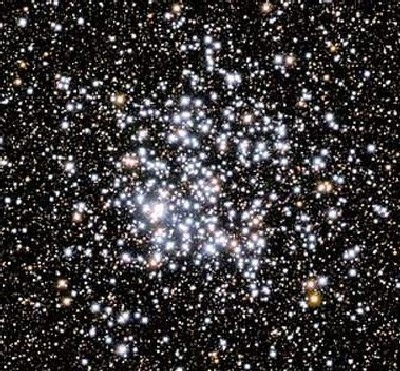
\includegraphics[width=0.4\textwidth]{pictures/РЗС.jpg}
    \end{figure}
\end{frame}


    \section{История}

    %-------------------------------------------------------------------------------------
    \section{Особенности строения}
    \begin{frame}
        \begin{itemize}
            \item Число звезд $\sim 10 \div 10^4$
            \item Как правило, состоят из~хорошо отличимого плотного ядра, окруженного более рассеянной <<короной>> из~звёзд
            \item Диаметр ядра $\sim 1$~пк
            \item Диаметр <<короны>> $\sim 10$~пк
            \item Плотность звезд в центре $\sim 40$~звезд/пк$^3$
            \item Часто вместе со скоплением наблюдается туманность
        \end{itemize}
    \end{frame}
    \begin{frame}
        \begin{figure}
            \centering
                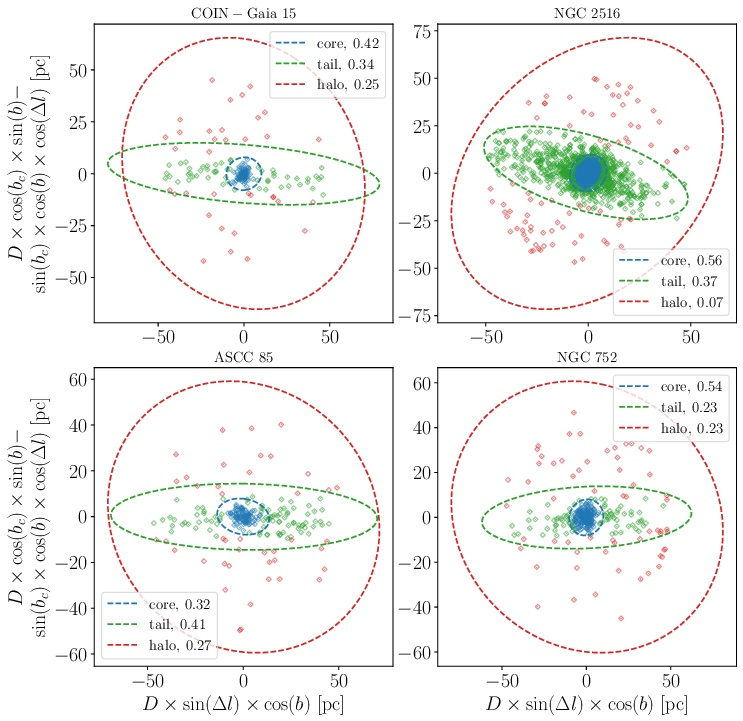
\includegraphics[width=0.6\textwidth]{pictures/Class1.jpg}
        \end{figure}
    \end{frame}
    \section{Основные способы классификации}
    \subsection{Классификация Шепли}
    \begin{frame}
        Простая схема классификации, предложенная Шепли в~его работе 1930 года\cite{ShapleyClass}.
        \begin{itemize}
        \item a --- Неровности поля
        \item b --- Звездные ассоциации
        \item c --- Очень рыхлые и~нерегулярные скопления
        \item d --- Рыхлые скопления
        \item e --- Среднебогатые компактные скопления
        \item f --- Достаточно богатые компактные скопления
        \item g --- Значительно богатые и~концентрированные скопления
        \end{itemize}
    \end{frame}
    \subsection{Классификация Трамплера}
    \begin{frame}
        Схема классификации, предложенная Трамплером в его работе 1930 года\cite{TrumpClass}. Состоит из трех частей.
        \begin{itemize}
            \item Концентрация
                \begin{enumerate}[I ---]
                    \item Отдельностоящий; сильная концентрация к центру
                    \item Отдельностоящий; слабая концентрация к центру
                    \item Отдельностоящий; нет концентрации к центру
                    \item Плохо отделен от окружающего звездного поля
                \end{enumerate}
            \item Диапазон яркости
                \begin{enumerate}[1 ---]
                    \item Небольшой диапазон яркости
                    \item Умеренный диапазон яркости
                    \item Большой диапазон яркости
                \end{enumerate}
            \item Богатство
                \begin{enumerate}
                    \item[p ---] Бедное (меньше $50$ звезд)
                    \item[m ---] Умеренно богатое (от $50$ до $100$ звезд)
                    \item[r ---] Богатое (более $100$ звезд)
                \end{enumerate}
        \end{itemize}
        Буква «n» после класса Трамплера указывает на то, что со~скоплением связана туманность.
    \end{frame}
    %-------------------------------------------------------------------------------------
    \section{Методы определения параметров РЗС}
    \subsection{Методы определения покраснений. Двухцветная диаграмма}
    \begin{frame}
        Основной способ определения избытка цвета РЗС.
        \begin{columns}
            % Column 1
            \begin{column}{0.5\textwidth}
                    \begin{itemize}
                        \item Типичная погрешность метода $\sim 0^m.01$
                        \item Избыток цвета определяется как сдвиг 
                            влево и вверх всей диаграммы скопления вдоль линии нарастающего покраснения до совпадения с последовательностью непокрасневших звёзд
                    \end{itemize}
            \end{column}
            % Column 2    
            \begin{column}{0.5\textwidth}
                \begin{figure}
                \centering
                    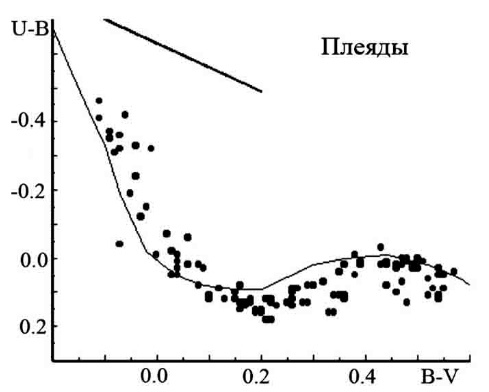
\includegraphics[width=0.9\textwidth]{pictures/Pl2Col.jpg}
                \end{figure}
            \end{column}
        \end{columns}
    \end{frame}
    \begin{frame}
        Применим не всегда.
        \begin{columns}
            % Column 1
            \begin{column}{0.5\textwidth}
                    \begin{itemize}
                        \item Всегда имеется трудность с~отделением членов скопления от~звёзд поля
                        \item У~заметного числа скоплений покраснения для разных звёзд не~равны --- имеется дифференциальное покраснение
                    \end{itemize}
            \end{column}
            % Column 2    
            \begin{column}{0.5\textwidth}
                \begin{figure}
                \centering
                    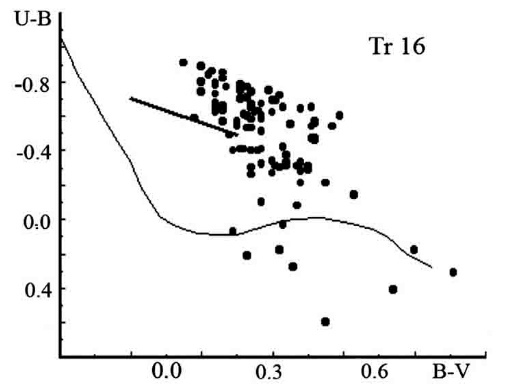
\includegraphics[width=0.9\textwidth]{pictures/Tr2Col.jpg}
                \end{figure}
            \end{column}
        \end{columns}
    \end{frame}
    \subsection{Методы определения покраснений. Q-метод}
    \begin{frame}

    \end{frame}
    \begin{frame}

    \end{frame}


    %-------------------------------------------------------------------------------------
    \section{Звездные ассоциации}
    
    \subsection{История открытия}
    
    \subsection{Характеристики}
    
    \subsection{Классификация}


    %-------------------------------------------------------------------------------------
    \section{Список литературы}
    \begin{frame}[t, allowframebreaks]{Список литературы}
        \bibliographystyle{plain}
        \bibliography{bibliography}
    \end{frame}
\end{document}